\documentclass{article}
\usepackage[utf8]{inputenc}
\usepackage{graphicx}
\usepackage{setspace}
\usepackage{amsmath}
\usepackage{geometry}
\title{ Assignment1}
\usepackage{float}
\author{Yang Yao }
\date{January 13th 2023}
\graphicspath{ {./images/} }
\geometry{a4paper,left=2cm,right=2cm,top=1cm,bottom=1cm}
\begin{document}

\maketitle

\section{Docker}
Install Docker and create image through Dockerfile.
Here is my what my Dockerfile looks like.
\begin{figure}[H]
\centering
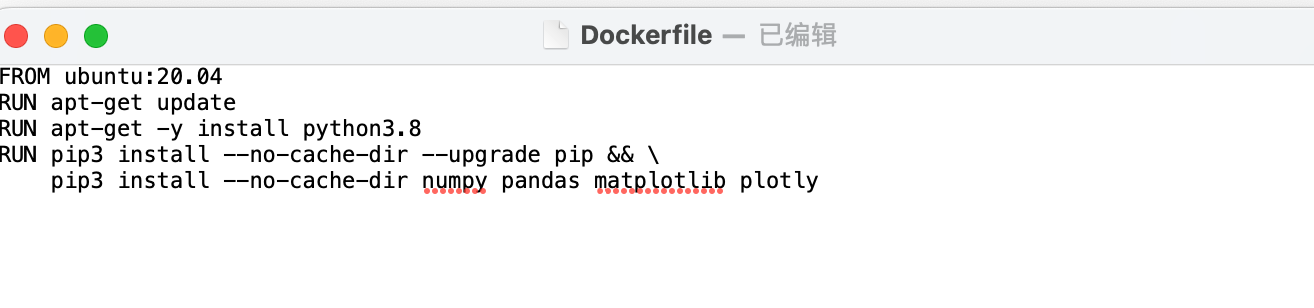
\includegraphics[width=15cm]{images/docker file.png}
\end{figure}

\noindent Then execute docker build command and now I have my image myimage:

\begin{figure}[H]
\centering
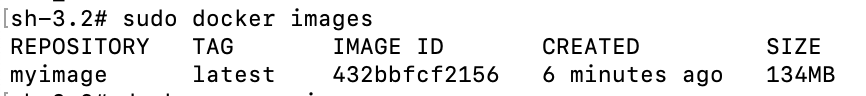
\includegraphics{images/image-images.png}
\end{figure}



\noindent Run the image and the container list is as shown below:
\begin{figure}[H]
\centering
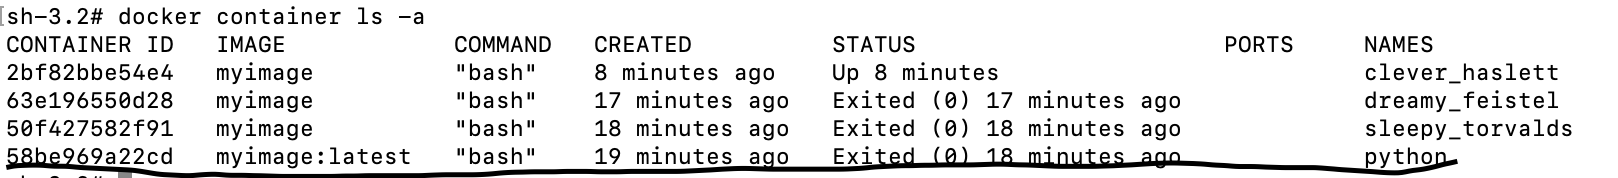
\includegraphics[width=15cm] {images/image-containers.png}
\end{figure}

\section{Identifying All Sets}
\subsection{question 1}
I use pandas library to solve the question. Use read\textunderscore csv function to read csv file and convert it to DataFrame. Then remove duplicate records and the rest are unique items. Next, I just have to count the number.
\begin{center}
\begin{figure}[H]
\centering
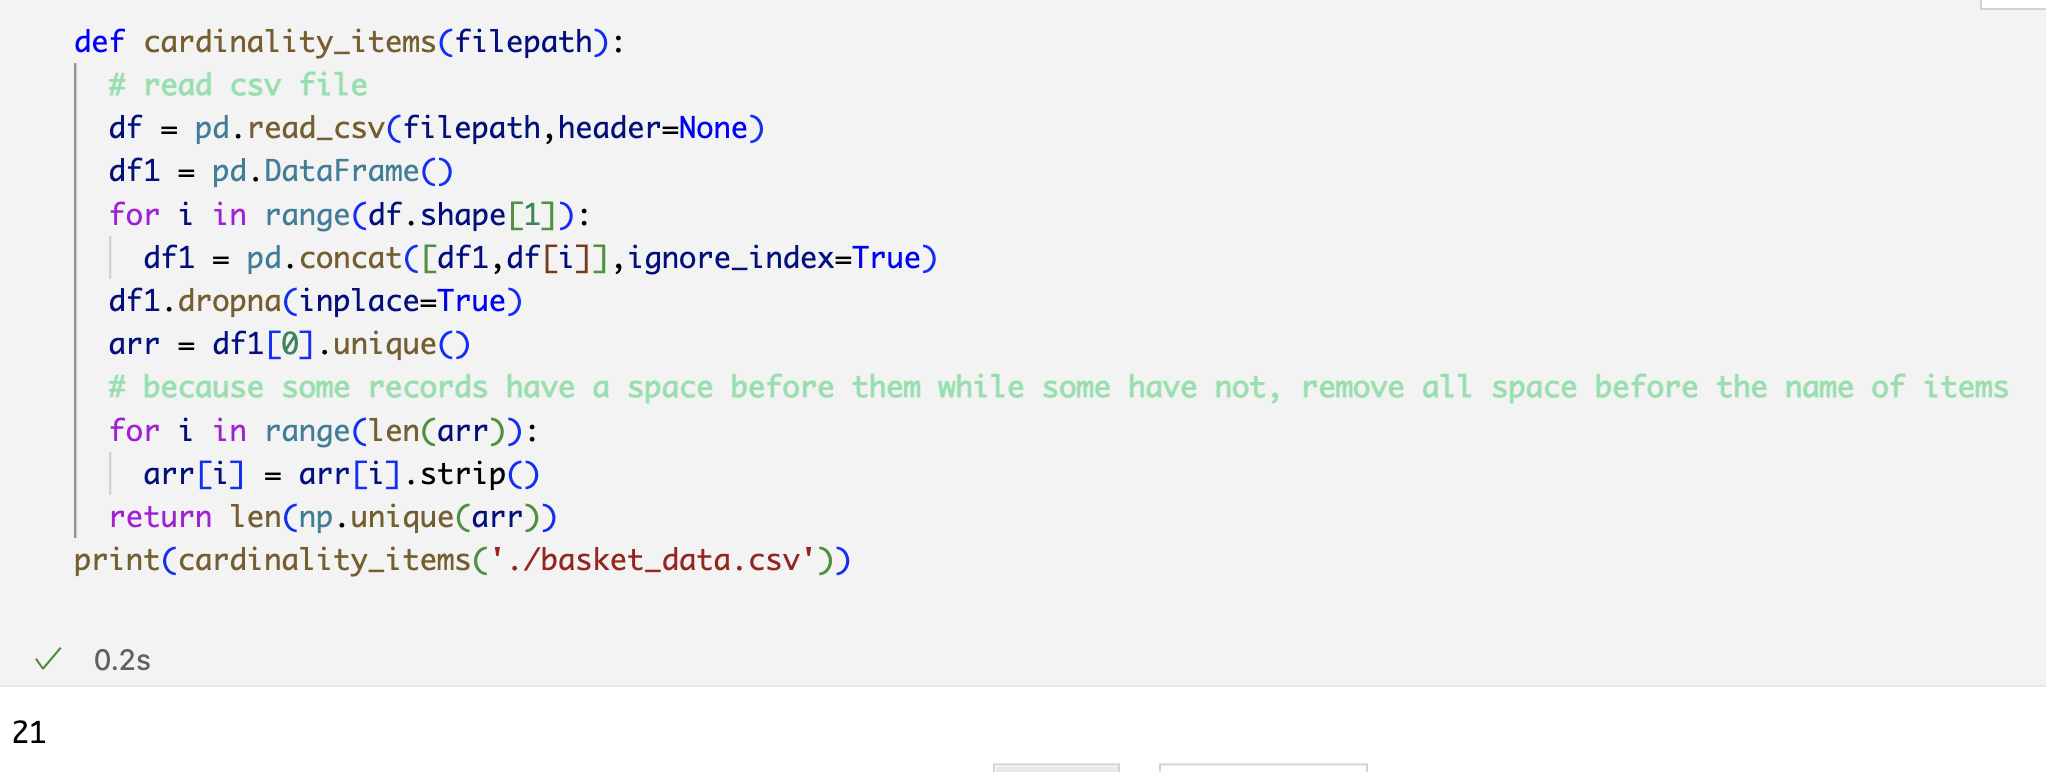
\includegraphics[width = 14cm]{images/cardinality.png}
\end{figure}
\end{center}


\subsection{question 2}
All possible sets that form by unique items is power set. The cardinality of power set of set of size \(n\) is \(2^n\).That is because every item in the set can be included or not included in a subset, so there are \( (\underbrace{2*2*2*...2*2}_{\text{Total\;n\;twos}}) = 2^n\) different subsets. 
\\ And because we are asked to ignore null set, so the number of sets with unique items can possibly be is \( 2^n-1\), where \(n\) is the number of unique items in the dataset.
\subsection{question 3}
To generate all possible subsets from N unique items, we should firstly deduplicate the dataset. And then, generate the power set of N unique items. Here I use itertools.combinations(S,n) function to generate all possible subsets with the size of n from set S. So I just need to generate all possible with the size from 0 to N, then I gain the power set.
\begin{center}
\begin{figure}[H]
\centering
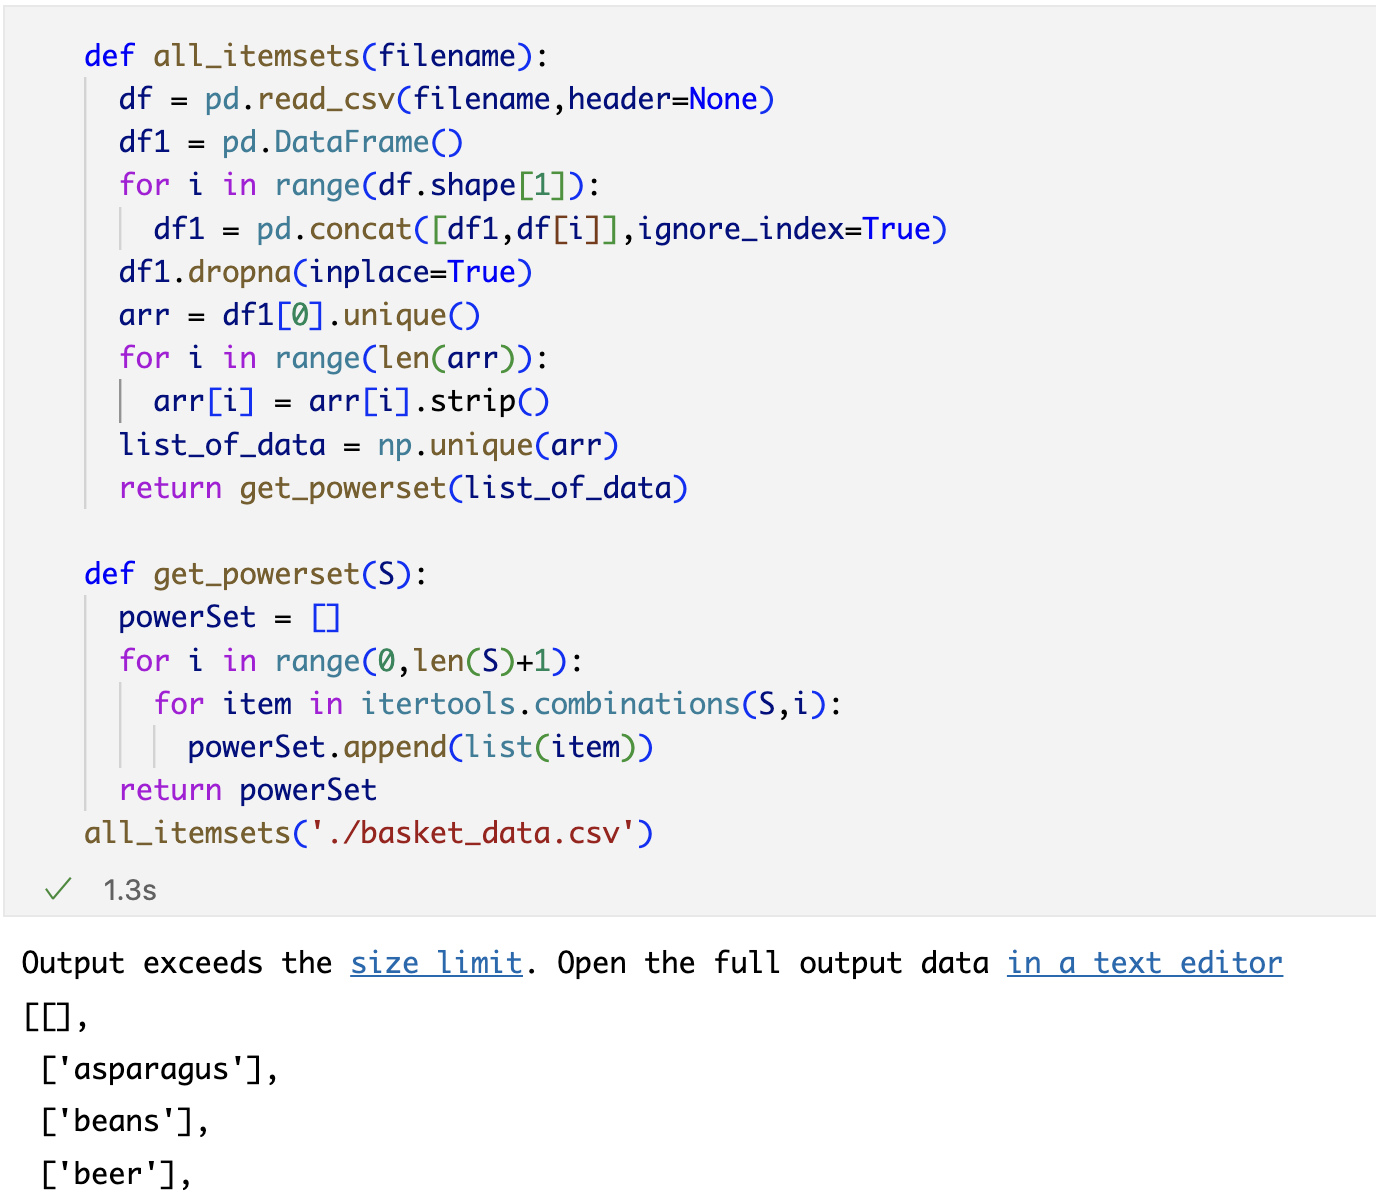
\includegraphics[width=14cm]{images/all items.png}
\end{figure}
\end{center}


\subsection{question 4}
Count the number of items in D and count the occurrences of S, then you get the probability. 
\begin{center}
\begin{figure}[H]
\centering
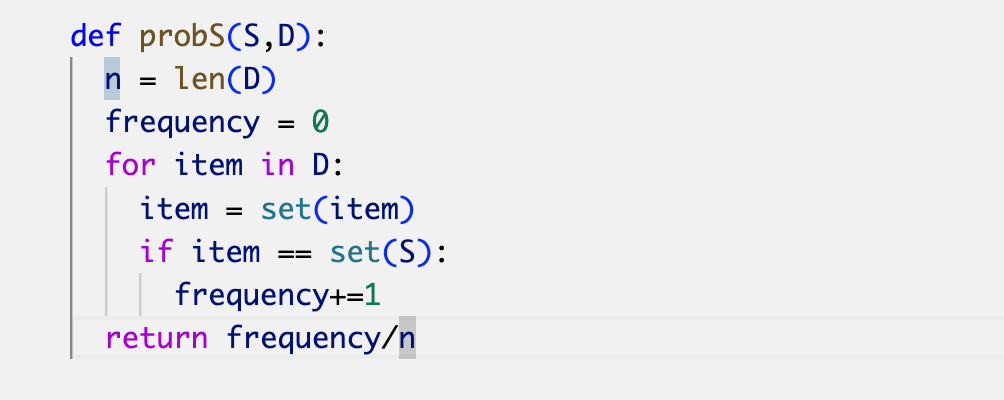
\includegraphics[width=13cm]{images/probS.png}
\end{figure}
\end{center}

\section{The Netflix Challenge}
\subsection{Data Verification}
As dataset description said, every data has 4 colons: MovieID, CustomerID, Ratting and Date. 
\begin{center}
\begin{figure}[H]
\centering
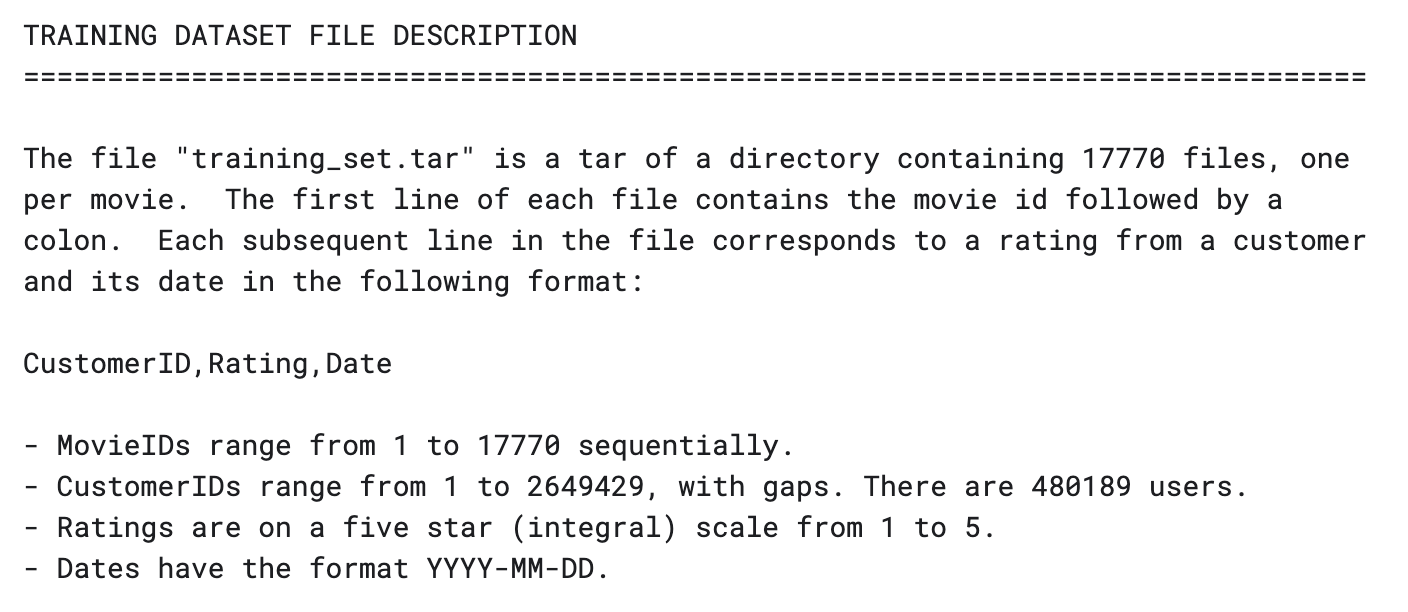
\includegraphics[width=13cm]{images/dataset_description.png}
\end{figure}
\end{center}

\noindent We can open the combined\textunderscore data1.txt and find the format is the same as description said. Then I load a part of data and preprocess the data to the format declared in the description, as shown below:
\begin{center}
\begin{figure}[H]
\centering
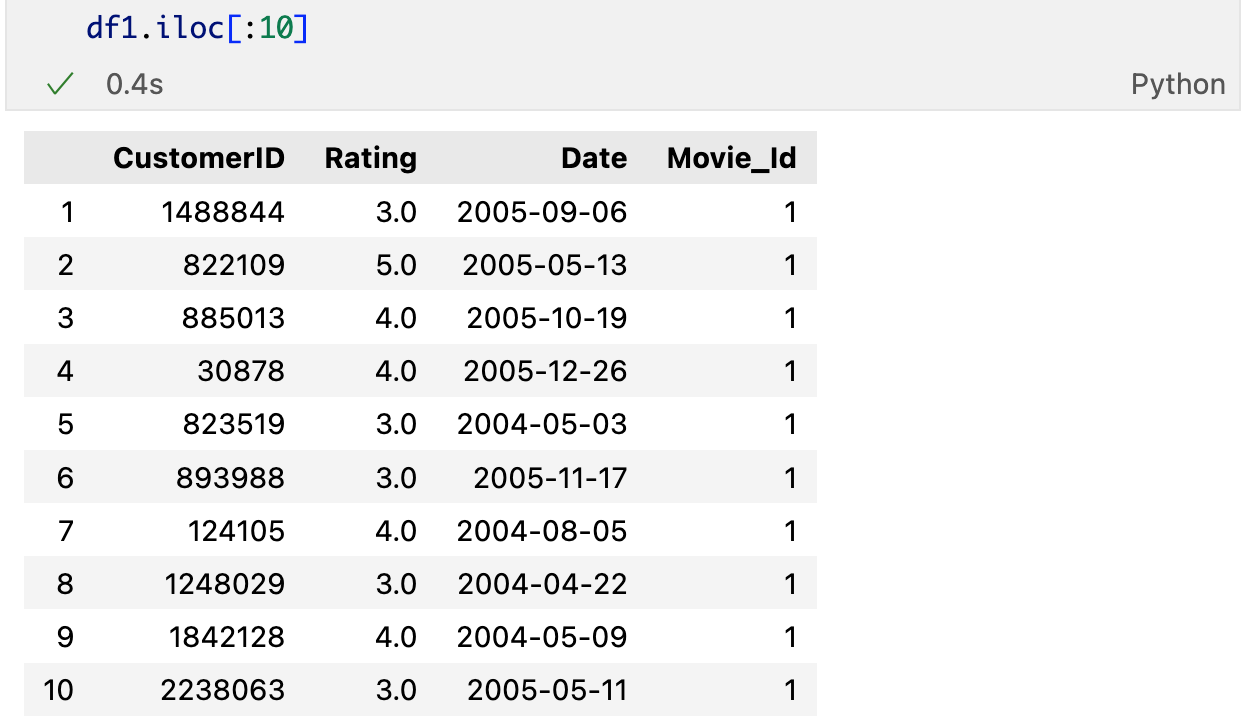
\includegraphics[width=13cm]{images/show_data.png}
\end{figure}
\end{center}

\subsection{Data Analysis}
\begin{enumerate}
{
\linespread{2.0} \selectfont
    \item \textbf{How many total records are there?}
}
\\
    There are totally 26847523 records.
    \begin{center}
    \begin{figure}[H]
    \centering
    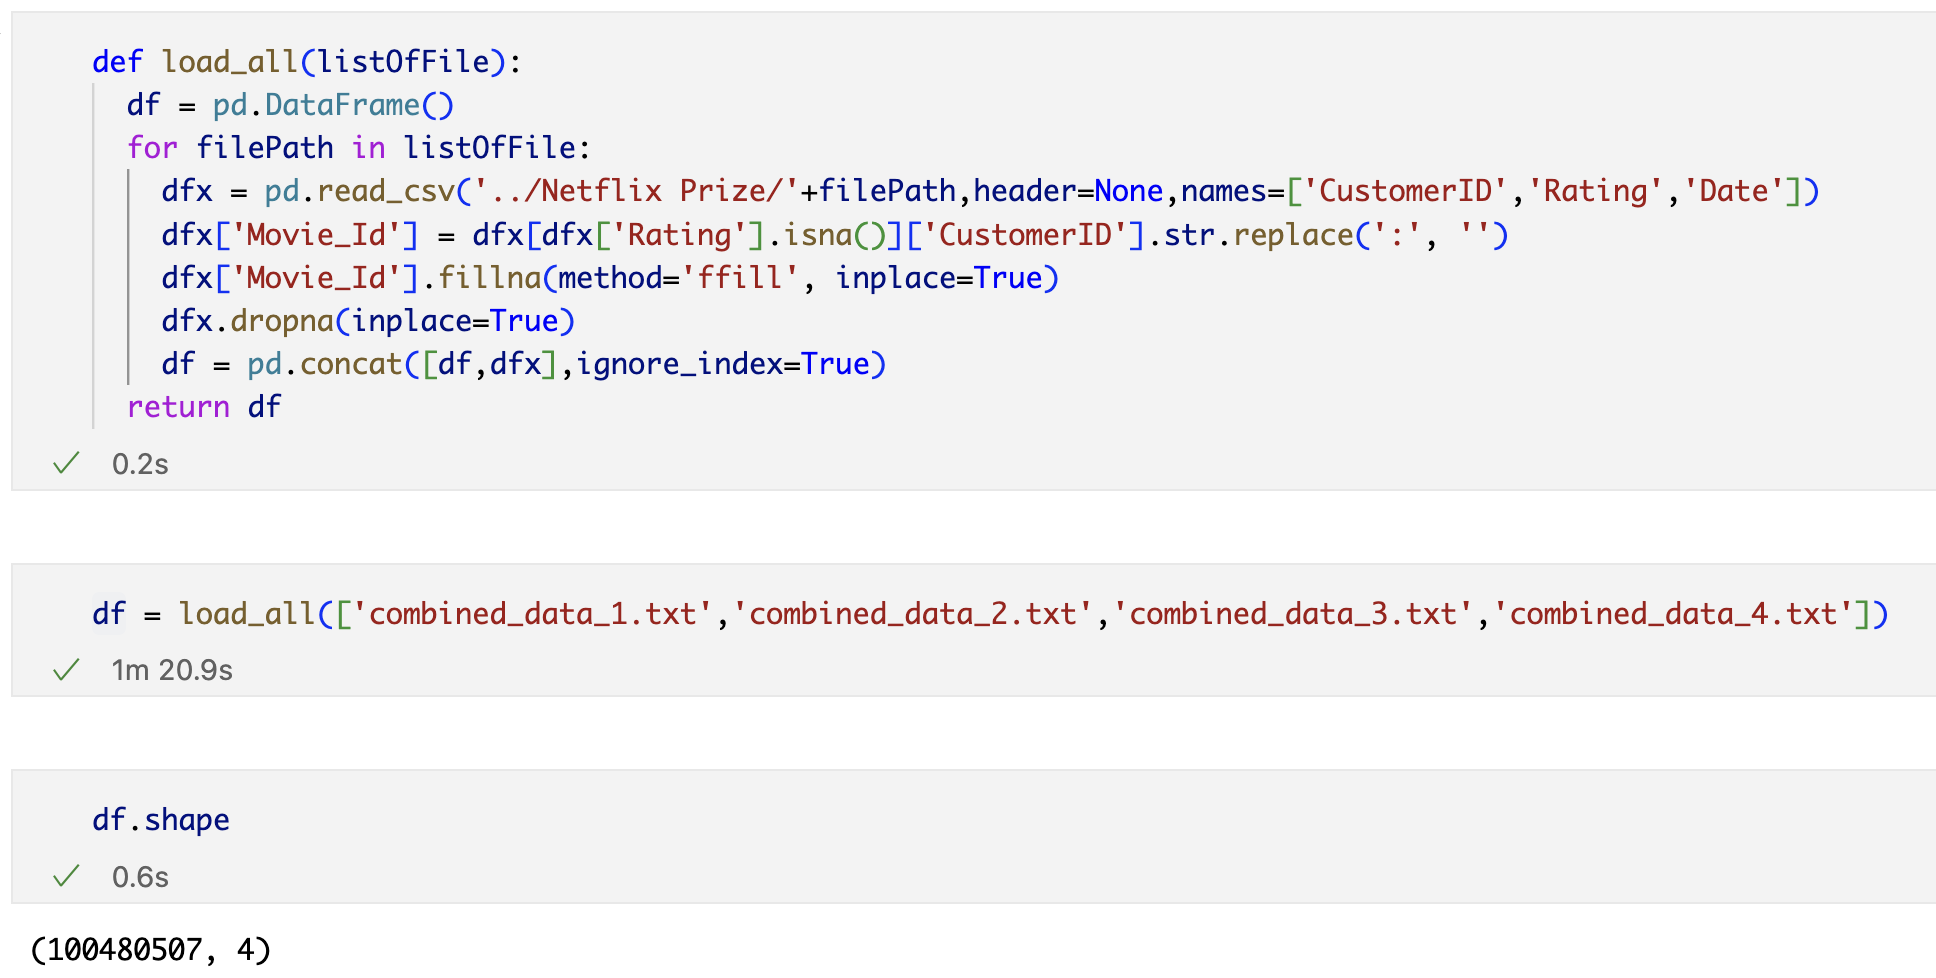
\includegraphics[width=14cm]{images/total data.png}
    \end{figure}
    \end{center}
{
\linespread{2.0} \selectfont
\item \textbf{Can you plot the distribution of star ratings over users and time?  The granularity of the sliding window is at your discretion. Are there any trends?}
}
To gain the distribution of ratings over time, group the rating by Date, then calculate average ratings for each Date:
\begin{center}
    \begin{figure}[H]
    \centering
    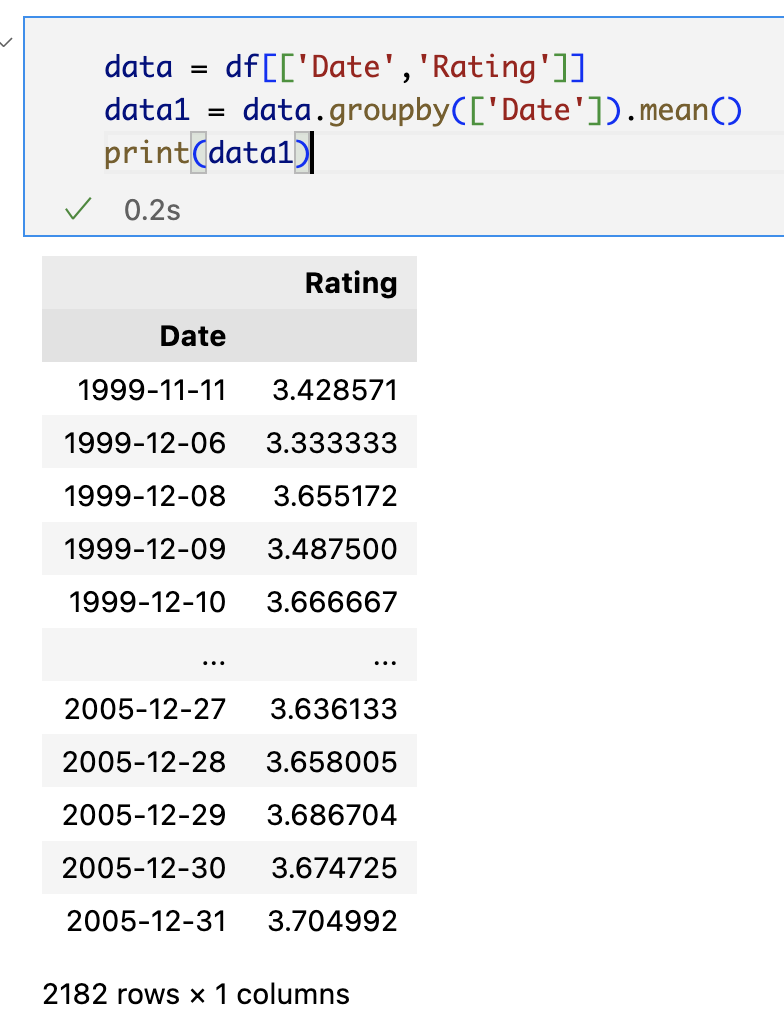
\includegraphics[height=10cm]{images/group by date.png}
    \end{figure}
\end{center}
\\ I plot the graph about the average rating stars over time, as shown below.

\begin{center}
    \begin{figure}[H]
    \centering
    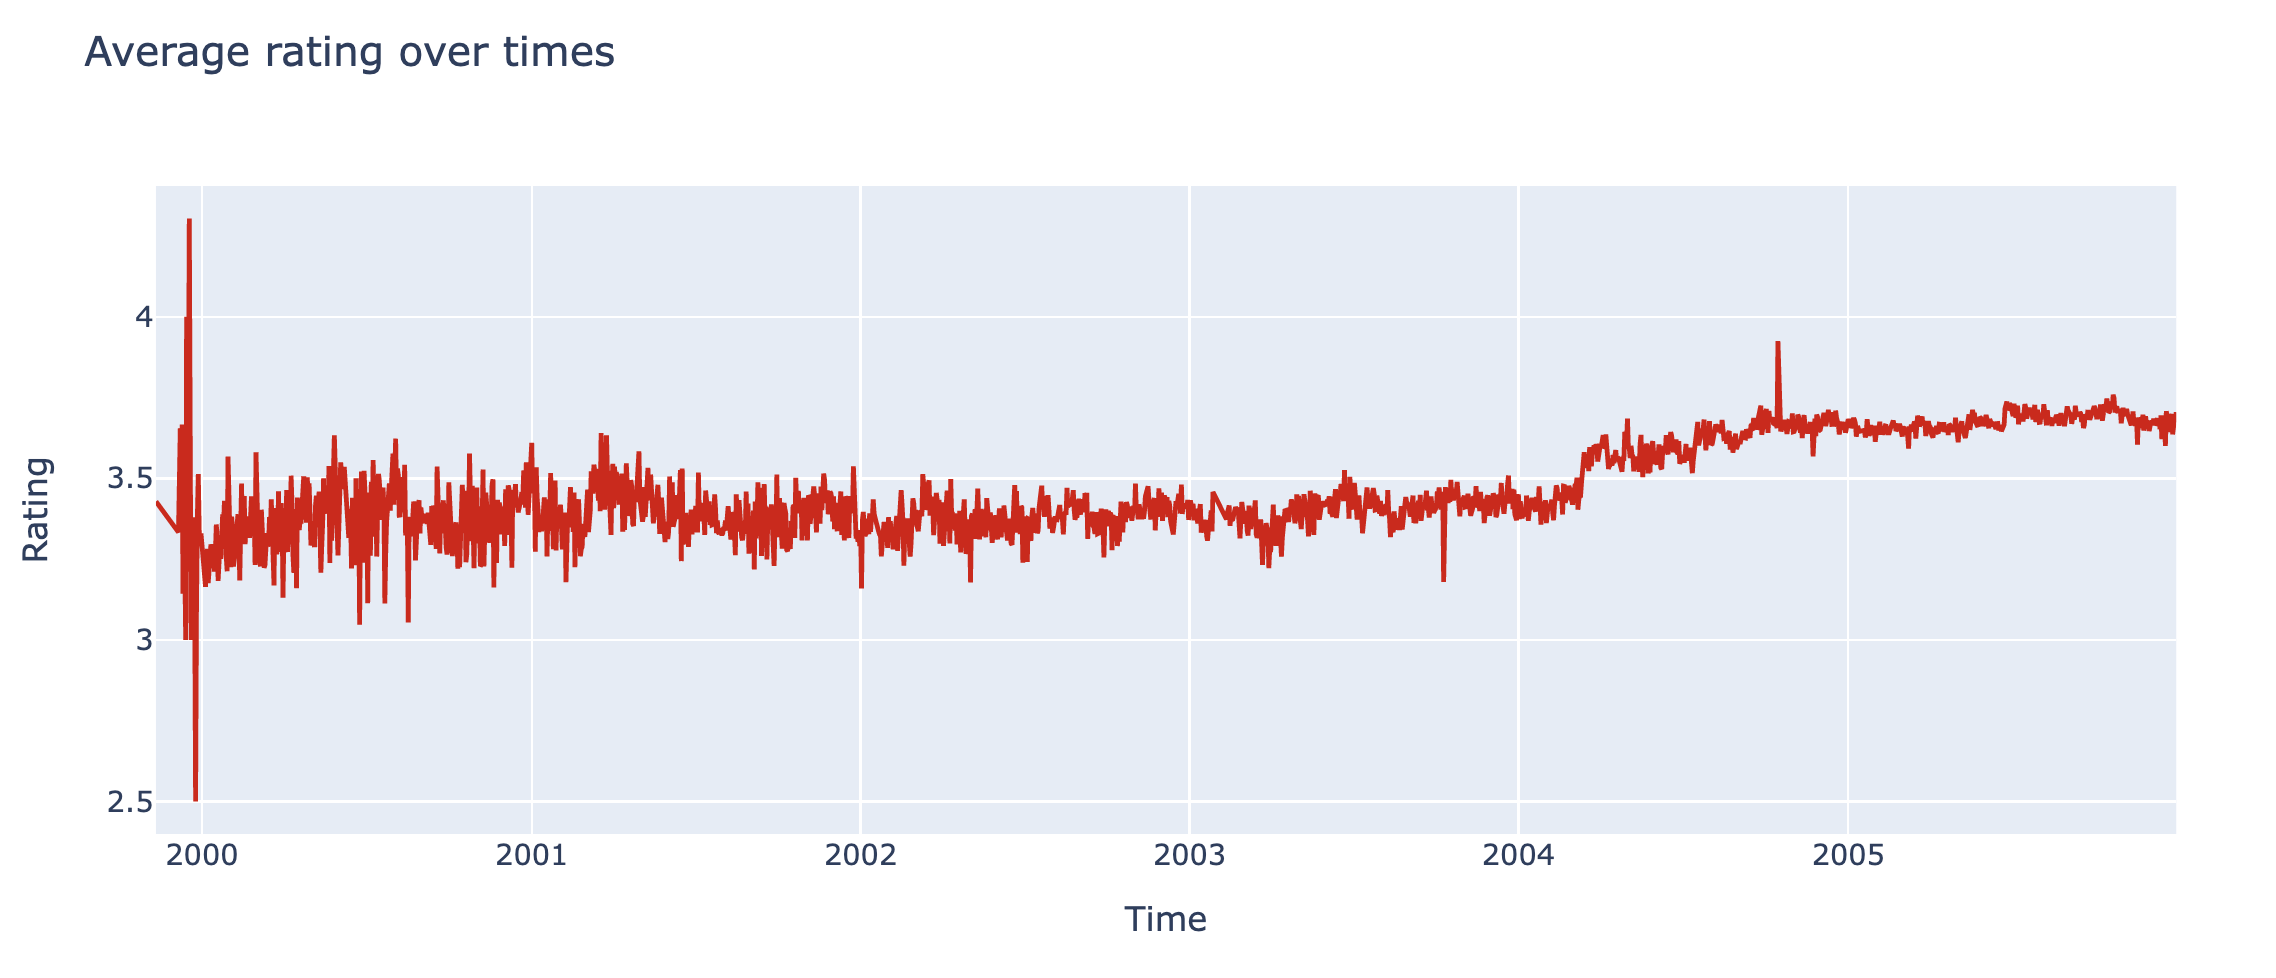
\includegraphics[width = 17cm]{images/rating over time.png}
    \end{figure}
\end{center}
{
\linespread{1.5} \selectfont
It shows the rating stars are shock greatly near 2000. I think might be some excellent movies come at the end of 1999 and soon after that, because customers had seen those excellent movies, later movies were rated low for their relatively low quality comparing to excellent movies released right before them. And after 2004, ratings start growing higher, smoother and show upward trend and at Oct 2004 reach regional peak. In total, the rating stars show a slow upward trend.
}

Also, I plot a histogram shows ratings over users. It shows most users rate 4 stars and 1 or 2 star rating is relatively rear.
\begin{figure}[H]
    \centering
    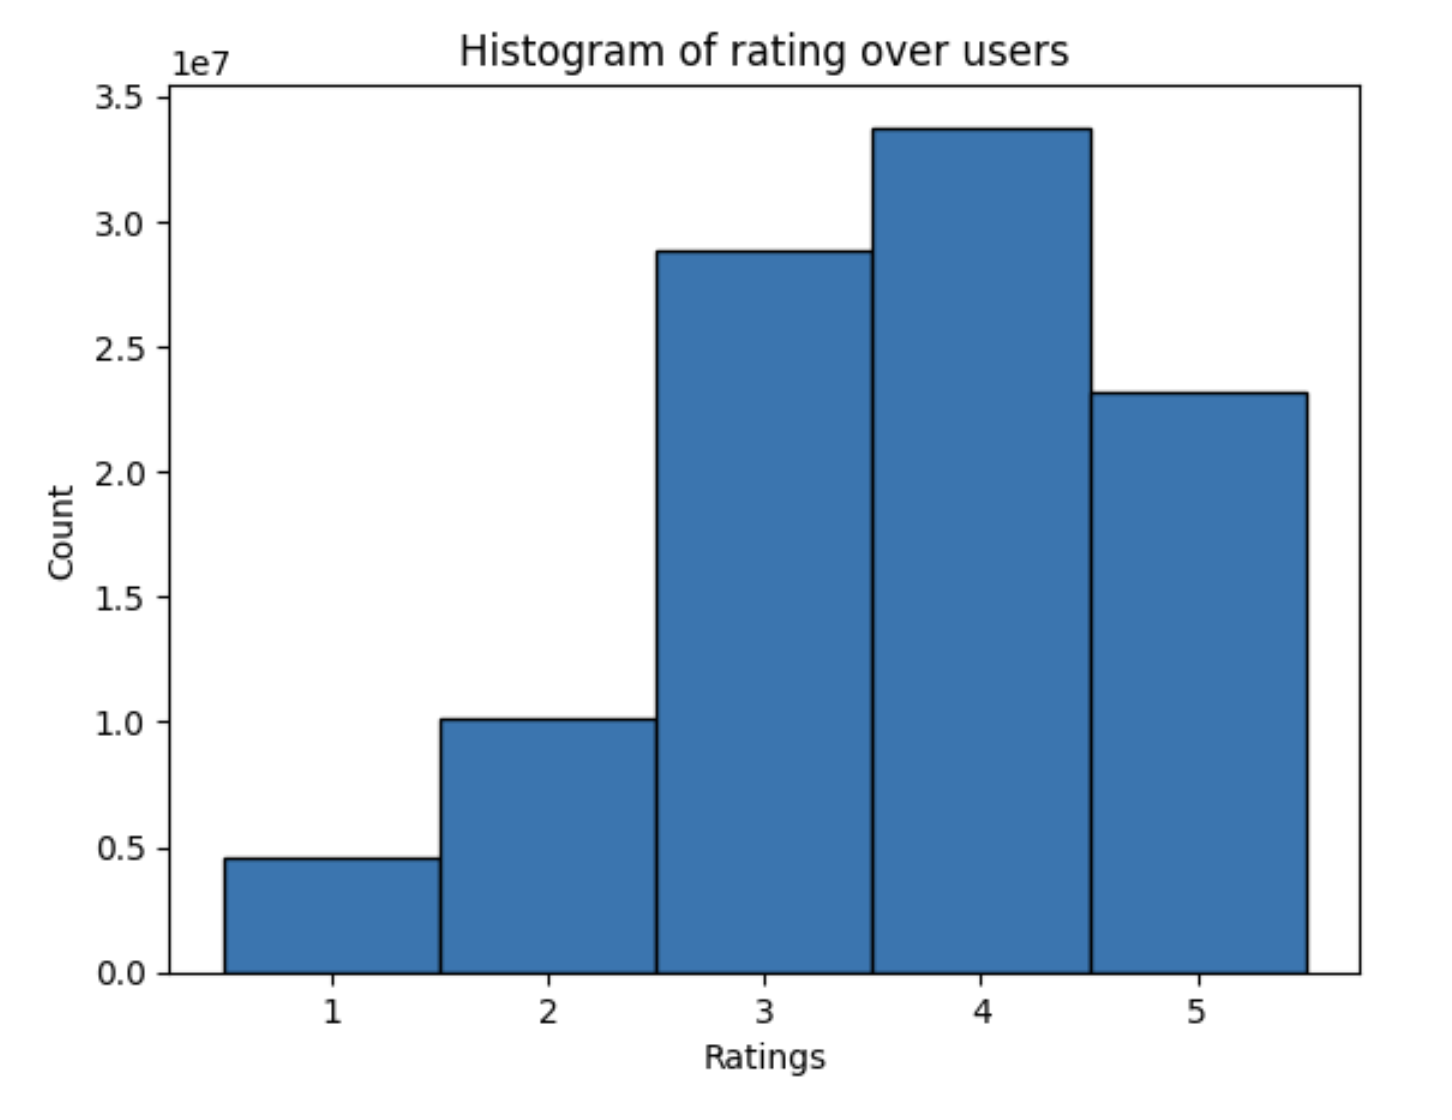
\includegraphics[width = 13cm]{images/ratings over user.png}
\end{figure}

\\
{
\linespread{2.0} \selectfont
\item \textbf {What percentage of the films have gotten more popular over time?}
}
\\
{
\linespread{1.3}\selectfont
There are about 64\% movies have gotten more popular over time. To clarify, a movie becomes more popular over time if the average film rating in the final year is greater than that of the first year. For example, if a movie got 3.5 stars on average in 2000 and 3.7 stars on average in 2004, I can say this movie have gotten more popular over the years. 
\\ To gain the answer, I round data info to year and group the data by MovieId and Date, then calculate it's mean. Then I get data as shown below:
\begin{figure}[H]
\centering
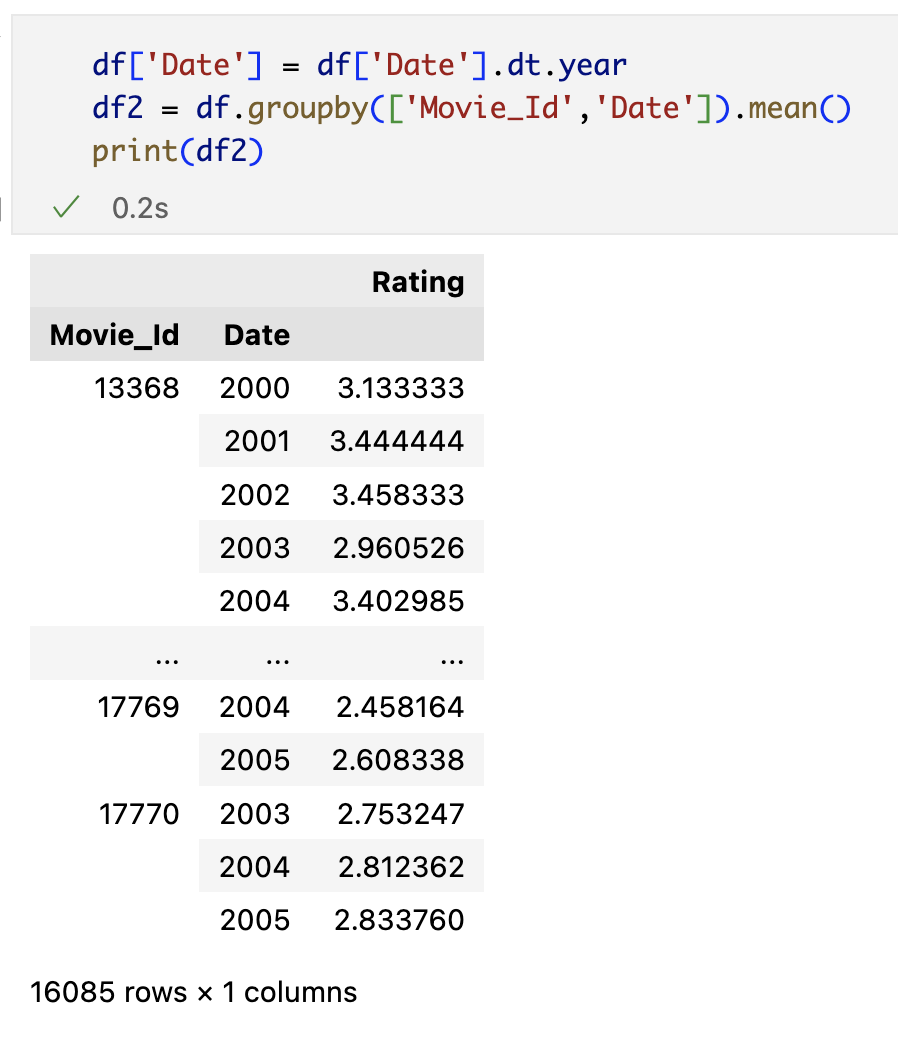
\includegraphics[width = 10cm]{images/group.png}
\end{figure}
\noindent Then I count how many movies got popular over time. I go through all MoiveId and check if its last year average rating greater than the first year. Finally, calculate the percentage:
\begin{figure}[H]
\centering
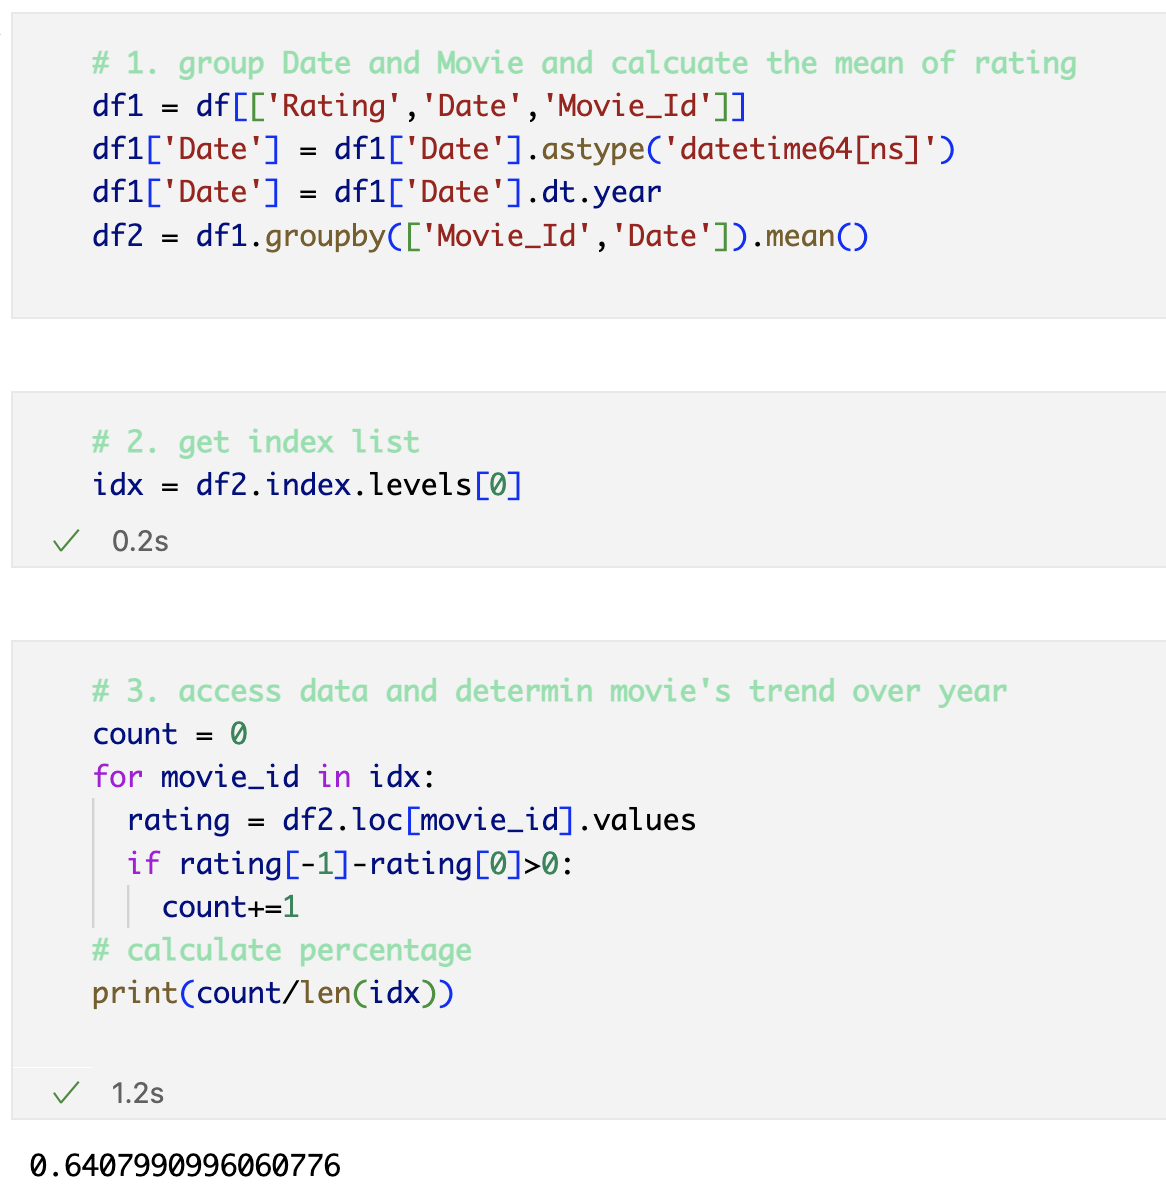
\includegraphics[width = 13cm]{images/percentage.png}
\end{figure}
}
{
\linespread{2.0} \selectfont
\item \textbf {How many films have been re-released? How do you know?}
}
{
\linespread{1.5}\selectfont
\\There are 369 movies have been re-released. If a movie has been re-released, it should have more than one record in the file "movie\textunderscore titles.csv" with the same name. So just have to count how many movie names have more than one record. By the way, the "movie\textunderscore titles.csv" is original a txt file and Kaggle convert it into csv file, but this causes some problems. The csv file use ',' to split data, but some movie name include ',', which leads some movies' name to be separated to several pieces and may lead to wrong answer. 
\\
\\Here I change "movie\textunderscore titles.csv" 's extension name to 'txt' and read raw data manually, then convert data to pandas DataFrame and execute groupby operation. Next just need to count how many movies meet the conditions. The code is as shown below:
}
\begin{figure}[H]
\centering
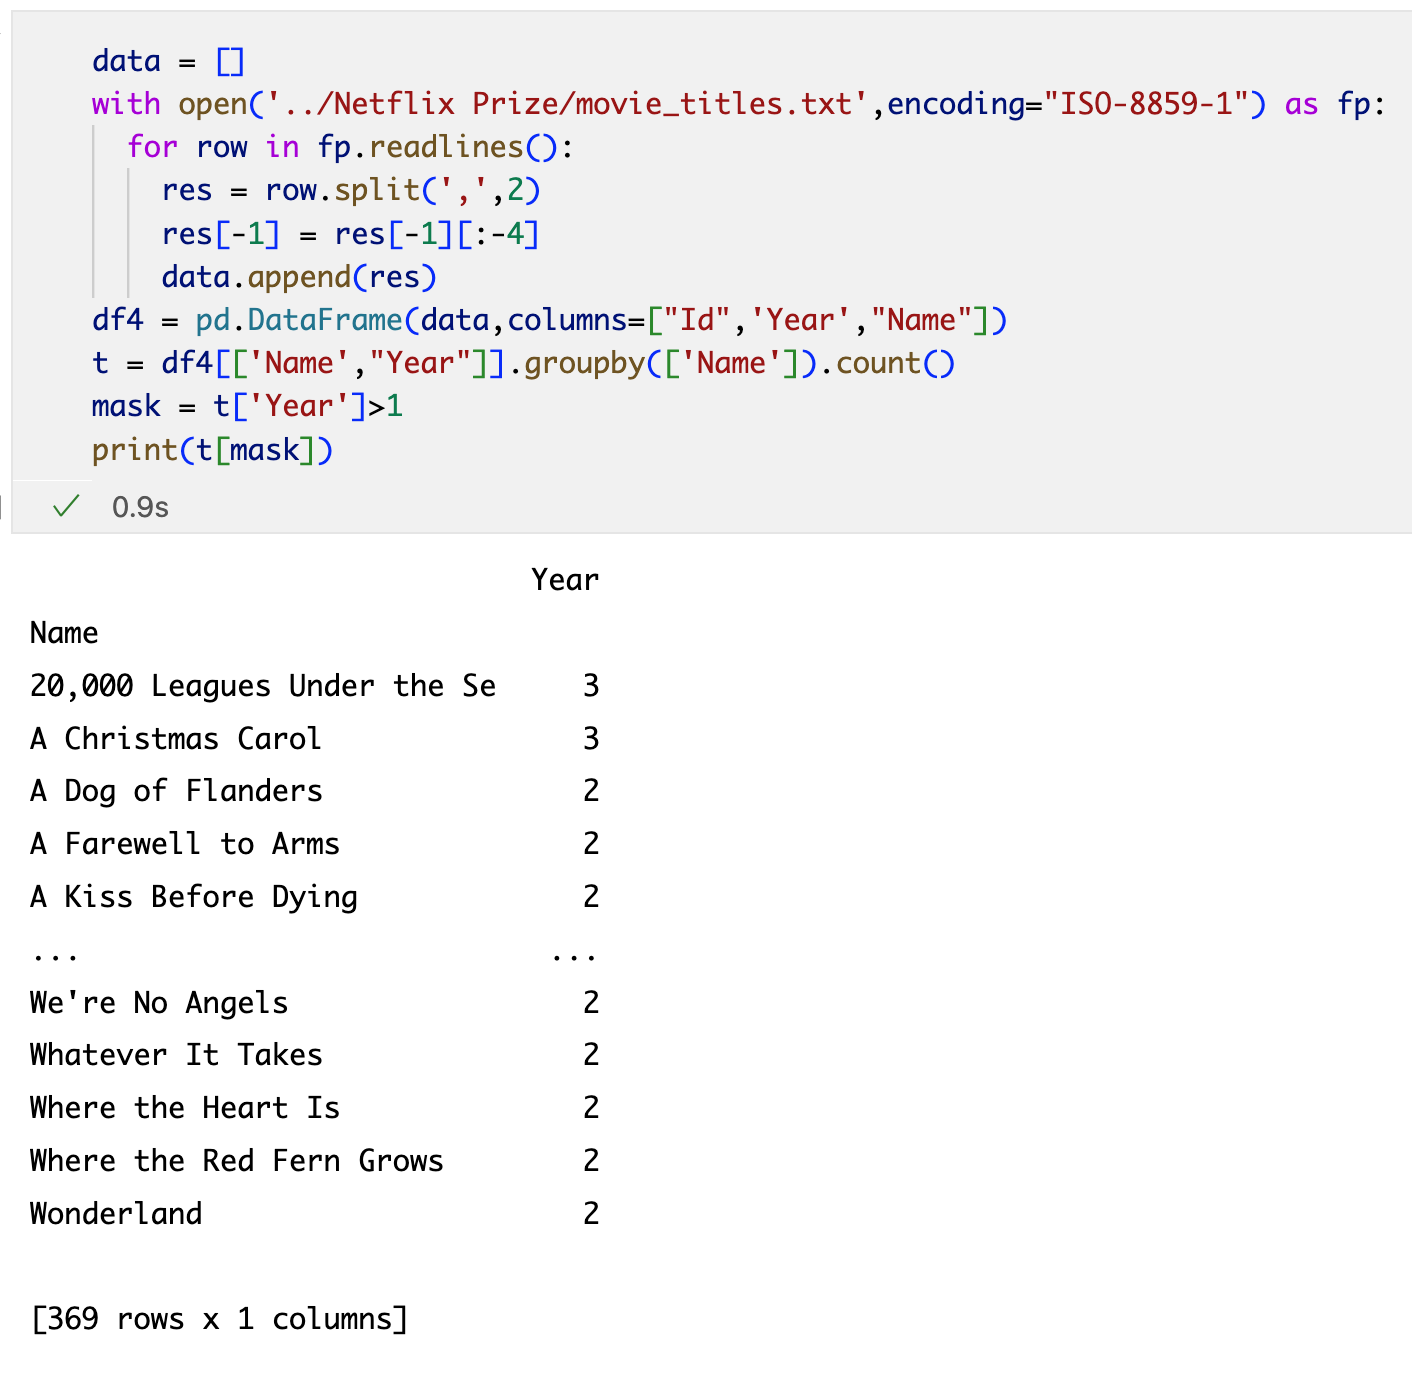
\includegraphics[width = 15cm]{images/5.png}
\end{figure}
{
\linespread{2.0} \selectfont
\item \textbf { What other information might we try to extract to better understand the data? For the questions that you may come up with (especially any time series data), make sure you back up your assertions with plots. Go ahead and play around with the data, and explore.}
}

\\I have tried to extract information of relation between rating stars and time since movies released. I merge combined\textunderscore data with movie\textunderscore titles so that we have information of released year for every movie. The data looks like below
\begin{figure}[H]
\centering
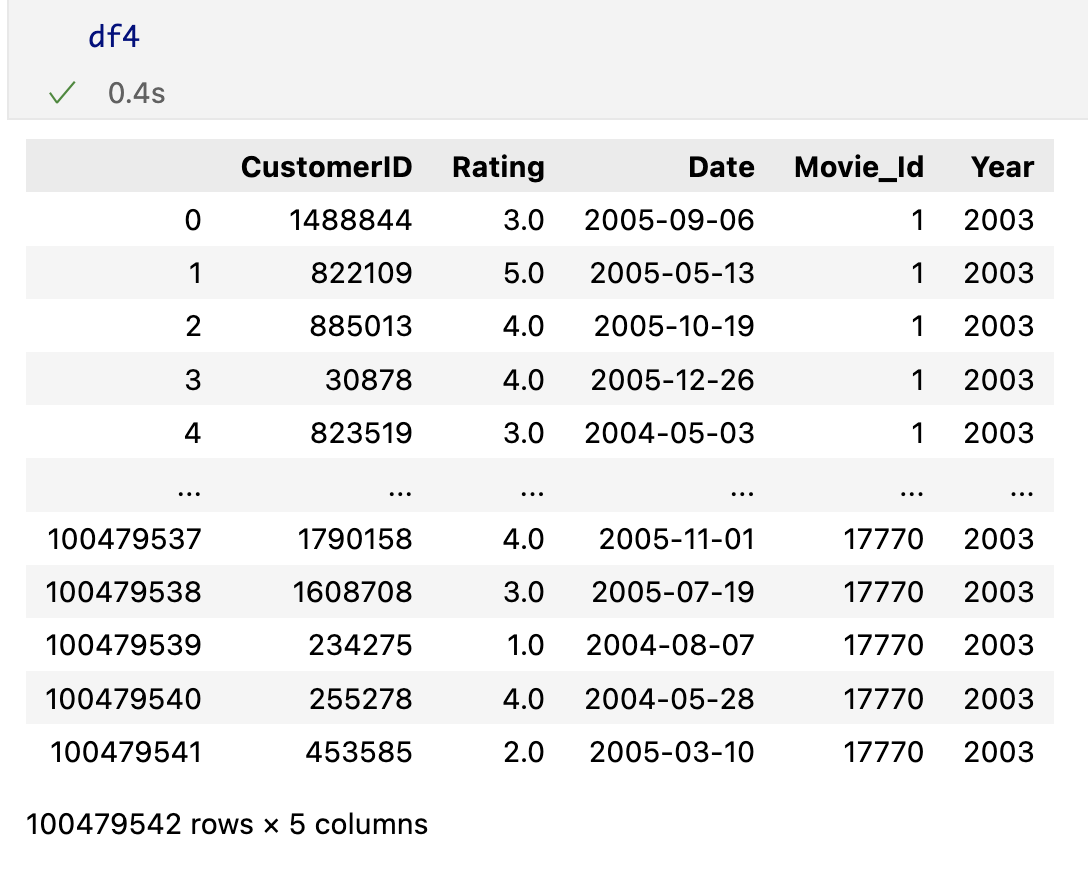
\includegraphics[width = 14cm]{images/merged data.png}
\end{figure}
Then we make difference between Date and Year, and calculate the mean then we get ratings over time since released\(:\)
\begin{figure}[H]
\centering
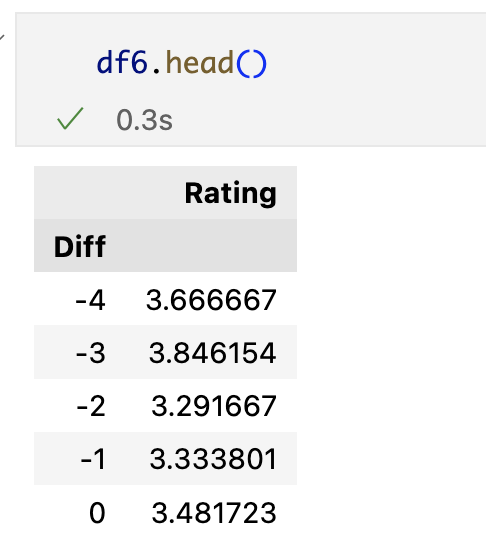
\includegraphics{images/df6.png}
\end{figure}
Finally, I plot a line to visualize the data\(:\)
\begin{figure}[H]
\centering
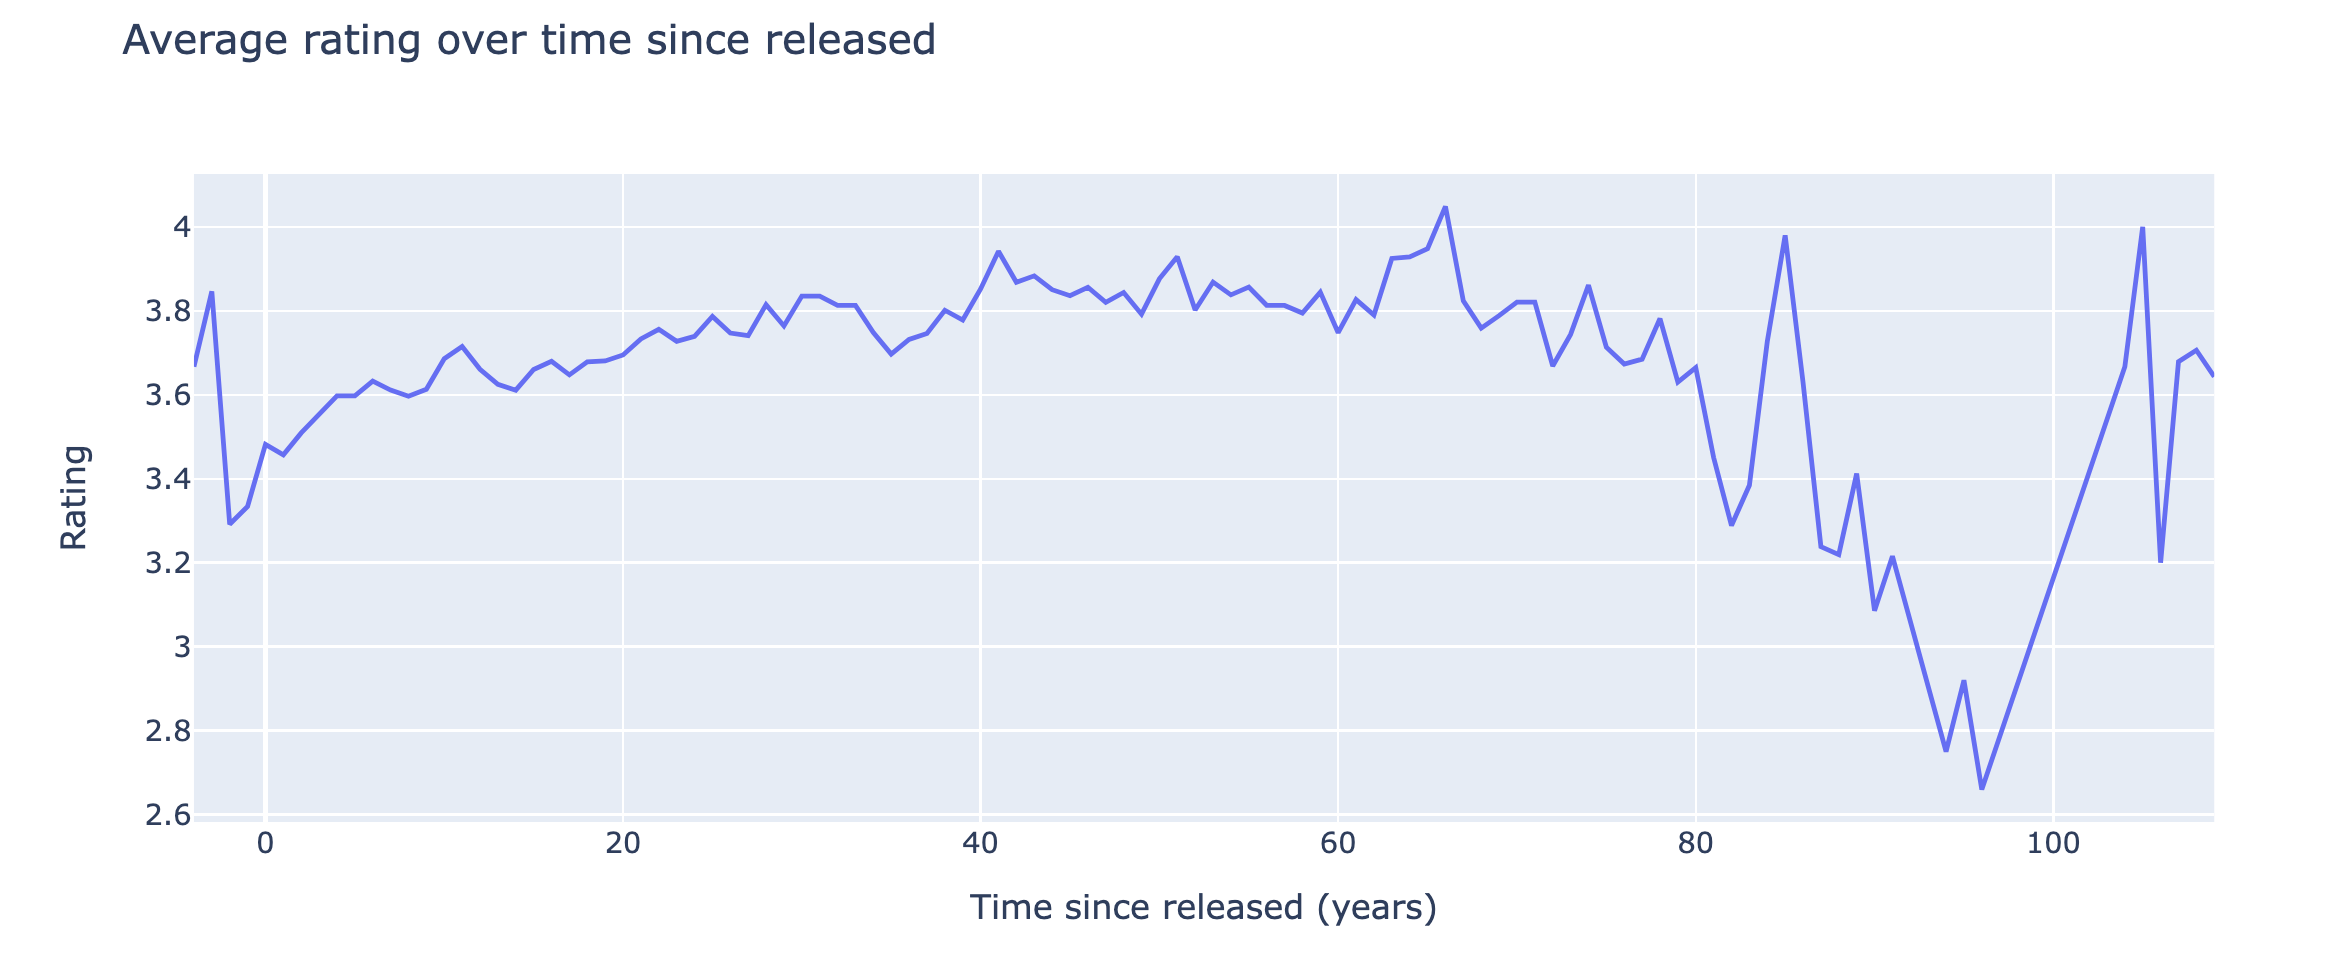
\includegraphics[width=18cm]{images/rating over time sine release.png}
\end{figure}
{
It shows that the ratings become higher as time since movie release increased in it's first 65 years. And an interesting thing is that the movies released 90 years ago are rated low, I think it might be movies at that time were early movies and were out of date for 21st century costumers. However, the movies released more than 100 years were rated relatively high, may be those movies are the very first movies and have important historical meaning, so audience rate high.
}
{
\linespread{2.0} \selectfont
\item \textbf {What are some interesting problems that we might solve? (No need to actually solve them!)}
}

{
\linespread{2.0} \selectfont
We might solve the problem of the trend of rating over time and users. So given a date and movie, we may use the thing we found before to predict what stars will a user most likely rates.
}
  
\end{enumerate}



\end{document}
